\documentclass[12pt, AofM.tex]{subfiles}




% \title{MATH598: A Review of Evolutionary Graph Theory}
% \author{Eoin O'Hearn}
% \date{\today}

\begin{document}

% \subfiletitle{A Review of Evolutionary Graph Theory}
% \newpage
% % \tableofcontents
% \newpage

% BIG PICTURE
% How do ideologies spread?
\section{Review of Evolutionary Graph Theory and Games on Graphs}
\subsection{Introduction}
The field of Evolutionary Graph Theory first arose with the seminal paper in 2005 titled "Evolutionary Dynamics on Graphs" by Lieberman et al. \cite{liebermanEvolutionaryDynamicsGraphs2005}. The authors seeked to understand how population structure would affect the evolution of newly arisen traits, either supporting their fixation or helping to drive them back to extinction. To study this behavior, homeogenous populations are generated with a neutral fitness equal to 1. Then an invader, or mutant, with fitness $r$ is randomly chosen to replace one of the individuals. Two nodes are then selected, one to reproduce and one to die, the graph is updated, and the process continues in this way until the mutants go extinct or reach fixation. See Figure \ref{overview} for an overview. The process is built upon an underlying stochastic structure that first appeared in Moran (1958) \cite{moranRandomProcessesGenetics1958}. The field has seen a continued surge of interest and new areas of study have explored in determining the computuational complexity of fixation probability problems, comparing update rules, calculating mean fixation time, and game theoretic extensions.

Game theory can be included with Evolutionary Graph theory by having nodes face strategic interactions with the neighbors. The payoff of the game then affects the nodes fitness and so strategy profiles can be dynamically evaluated on the graph's structure. Studying evolutionary stable strategies is a central problem in evolutionary biology. Organisms, in their fight for survival, can be viewed as playing different strategies to maximize their chances at aquiring resources or minimizing energy expendtiture. A classic example of this is the 'Rock-Paper-Scissors' game represented by the sexual strategies of the male Side-blotched lizards (\emph{Uta spp.}) \cite{sinervoRockPaperScissors1996}. In this lizard, there exists three different throat-colors, orange-throated, yellow-throated, and blue-throated. Each color attempts to mate and reproduce via specific strategies. The orange-throated males are aggressive and establish large territories. Yellow-throated males are also known as sneaker males because of their tendency to sneak into the territiories of the orange-throated males and mate with the females. The blue-throated males defend just one or two female mates, but are able to defend against sneaker attacks.

\begin{figure}
    \centering
    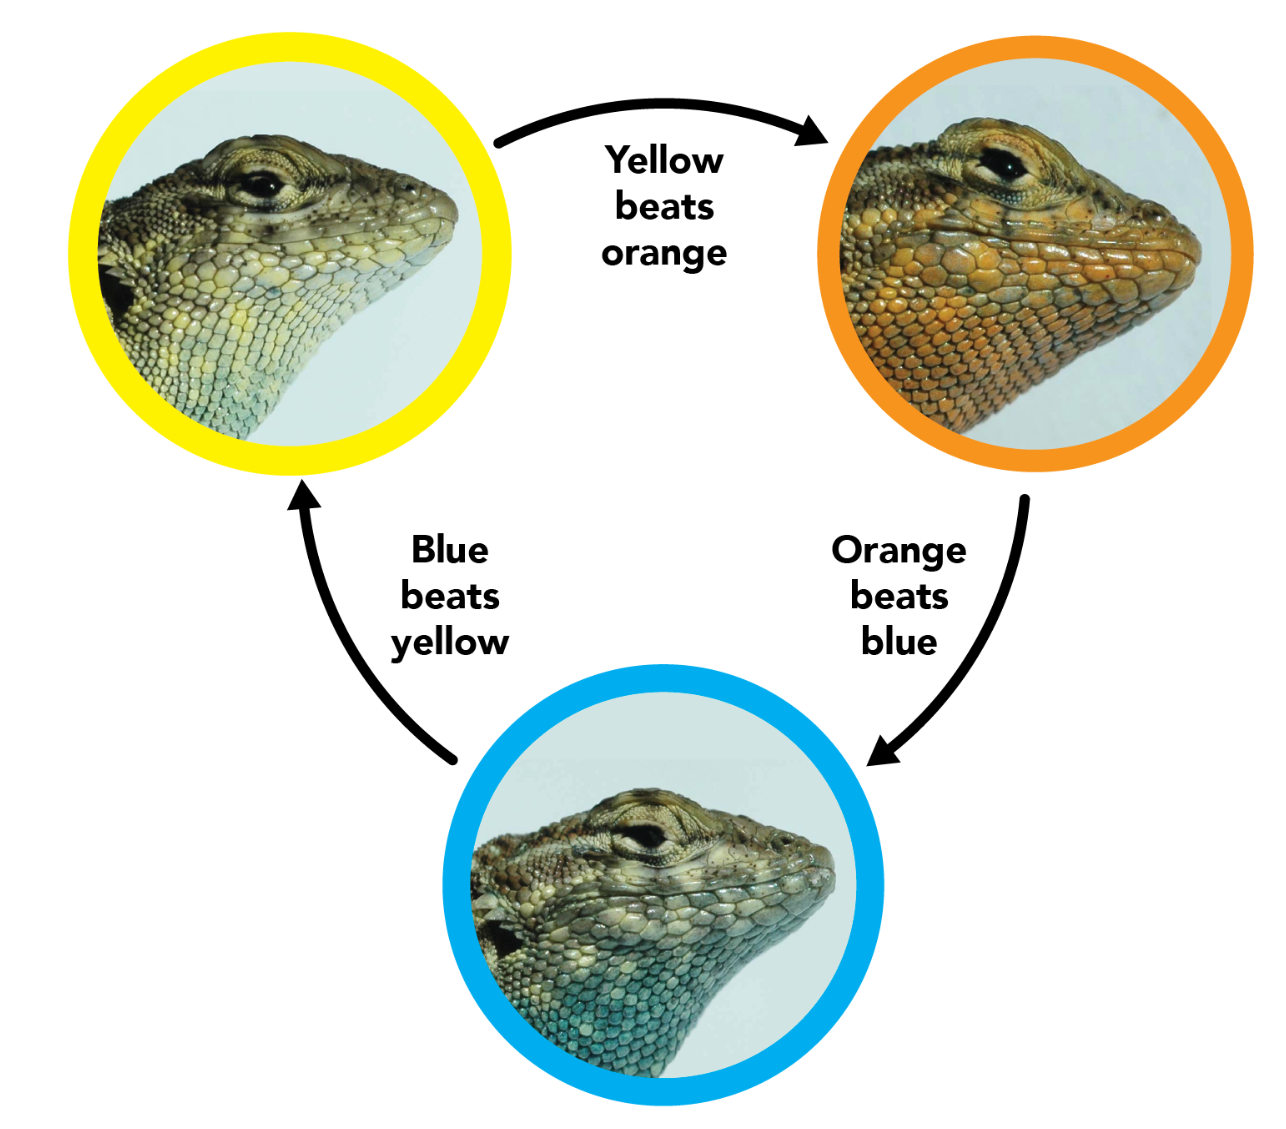
\includegraphics[width=0.5\textwidth]{img/lizard-rps.png}
    \caption{Dynamic relationships between different color morphs. Reproduced from \cite{UnderstandingEvolution}}
\end{figure}

These strategies are all face frequency-dependent selection. It is more advantageous to be a rarer morph than to be playing the same strategy of the other male lizards. This type of selection has led to a six-year period in which the percentage of different color morphs in the population oscillate around each other, hence the reference to rock-paper-scissors: orange beats blue which beats yellow which, in turn beats orange, and so no single strategy can reach fixation in the population.

In this case, the forces driving the favorable selection is apparent, but for many other extant strategies this is not true. Classical evolutionary theory seems to not allow for the selection of non-selfish behavior. In 1964, W.D. Hamilton introduced the idea of 'inclusive fitness' \cite{hamiltonGeneticalEvolutionSocial1964}. This led to the development of "Hamilton's rule" that defined mathematically the situations in which cooperative behavior would be favored by natural selection. Let $r$ be the relatedness between two individuals, $b$ the benefit of cooperative behavior, and $c$ the cost to the helper. If the following relationship holds, then organisms will act altruistically,
\begin{equation}
    rb > c
\end{equation}   
We can extend this idea to general populations of organisms by playing the "Prisoner's Dilemma" game on an Evolutionary Graph. In the famous game theory problem, individuals choose to either cooperate or defect. Their playoff is determined by both the strategy they choose and the strategy chosen by their opponent. Cooperators choose to help and incur a cost in doing so, while defectors solely benefit. Ohtsuki et al. found that cooperation was favored by selection when the benefit-to-cost was higher than the average degree of the graph, $k$ \cite{ohtsukiSimpleRuleEvolution2006}.
\begin{equation}
    \frac{b}{c} > k
\end{equation}
This relationship was shown to exist in population structure of primates and so may have contributed to the selection of cooperative behavior. Voelkl and Kasper (2009) analyzed the interaction dynamics of 70 different primate groups \cite{voelklSocialStructurePrimate2009}. They found that the resulting graph followed the benefit-to-cost ratio rule from \cite{ohtsukiSimpleRuleEvolution2006}.  

This paper reviews the main findings of Evolutionary Graph Theory and formalizes the inclusion of game theoretic strategic interactions. It finishes with a discussion on numerical simulations and evidence for benefit-to-cost ratio rule being necessary, but not sufficient, for the fixation of cooperation in a population. 

% Since Dawkins first popularized the idea of the 'selfish gene' in 1976, the existence of cooperative behavior has been puzziling \cite{Dawkins:1976}.
\begin{figure}
    \centering
    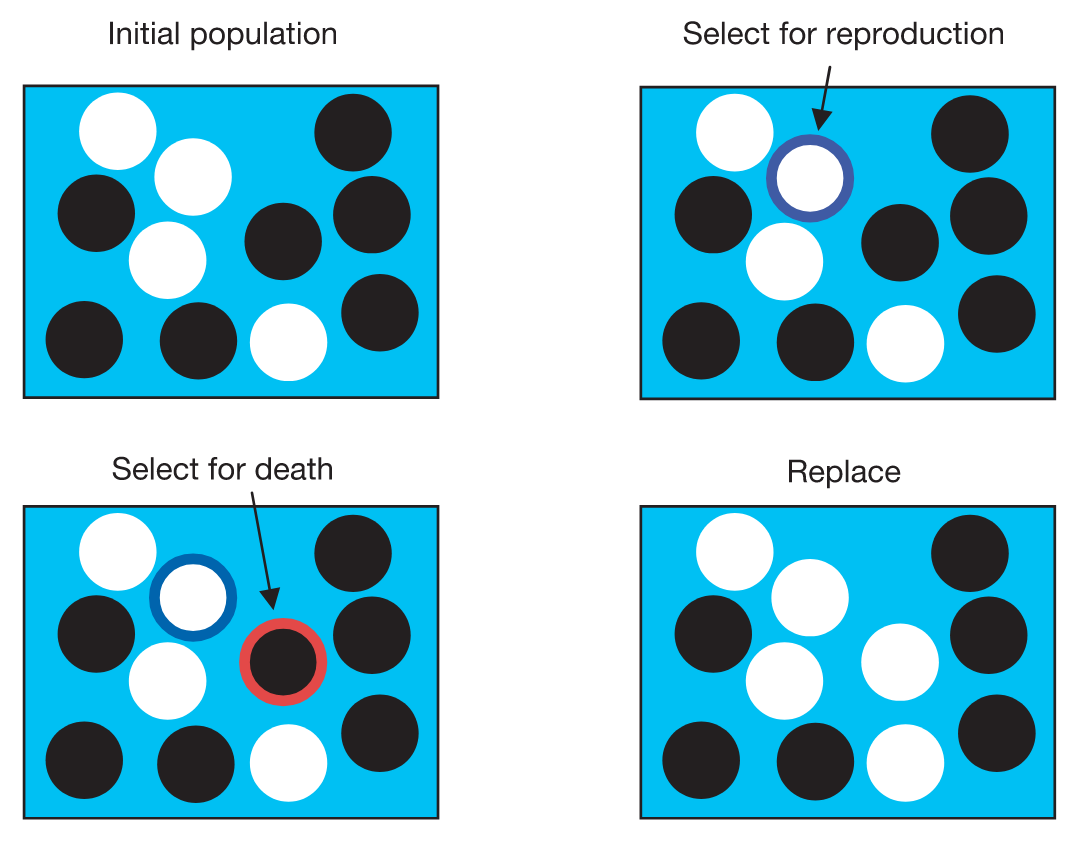
\includegraphics[width=0.5\textwidth]{img/overview.png}
    \caption{Updating an Evolutionary Graph. Reproduced from \cite{liebermanEvolutionaryDynamicsGraphs2005}}
    \label{overview}
\end{figure}

\newpage

\subsection{Evolutionary Graph Theory}

 
\begin{definition}
    A population $V$ is a set of $N$ individuals,$\{v_1, \ldots, v_N\}$, along with a fitness mapping $f: V \rightarrow \mathbb{R}$ such that $f_i = f(v_i)$ is the fitness of individual $i$. We say that an individual is a resident if $f_i = 1$ and a mutant otherwise, $f_i \neq 1$.  
\end{definition}

\begin{definition}
    An evolutionary graph $G$ is a population $V$ with adjacency matrix $W$ such that $\sum_j w_{ij} = 1 \; \forall \; i$. 
\end{definition}

As the reader might be able to guess based on the stipulation on the sum of the rows, we can consider evolutionary graphs to be a stochastic process. At each time step, an \emph{update rule} is used to determine which vertices, or individuals, are chosen for birth and death. The simplest such update rule, Birth-Death with Birth bias (BD-B), is introduced and used in \cite{liebermanEvolutionaryDynamicsGraphs2005}. In this update rule, one first picks vertex $v_i$ with probability proportional to $f_i$. Then vertex $v_j$ is chosen from the neighbors of $v_i$ with probability $w_{ij}$ from the adjacency matrix. Lastly, $v_i$ replaces $v_j$ so that $v_j$ is now identical to $v_i$, but still a separate node, or individual. 

This is, however, just one such update rule that can be used when studying evolutionary graphs. There exists three main families of update rules. BD-B is part of the Invasion Process family (IV), where the first node chosen replaces the second. The reverse, where the second node chosen replaces the first and so $v_j$ would replace $v_i$, constitutes the aptly named Voter model family (VM). The last family focuses on choosing edges rather than nodes, and so is named Link Dynamics (LD). In this family of update rules and edge is first selected between nodes $v_i$ and $v_j$. Then, one node is chosen to replace the other depending on what bias rule is being used. 

Reviewing the first update rule, BD-B, the first node is chosen with probability proportional to its fitness, but the fitness of the node chosen to 'die' is not considered. There exists a fitness bias on the node chosen to reproduce, hence a \emph{Birth} bias. But we could easily choose to instead consider put the bias on the node chosen to die using a probability distribution inversely proportional to its fitness, where a low fitness would increase the probability of being chosen for death. 


The possible biases are further outlined in Table \ref{bias-table} for the Birth-death update rule, but are analagous for the other families, with one exception. When using a Link Dynamic update rule, it is possible to have an Imitation bias such that whichever node of the selected edge has the higher fitness is chosen to reproduce.    

\begin{table}
    \centering
    \caption{Possible biases with Birth-death update rule.}
    \label{bias-table}
    \begin{tabularx}{\textwidth}{c | X}
        \hline
        Bias & Process \\
        \hline \hline
        Unbiased and undirected & Pick $v_i$ and $v_j$ with uniform probability \\
        Directed & Pick vertex $v_j$ with probability proportional to outgoing edges of $v_i$ \\
        Birth-bias & Pick vertex $v_i$ probability proportional to $f_i$ \\
        Death-bias & Pick vertex $v_j$ probability proportional to $f^{-1}_i$ \\
    \end{tabularx}
\end{table}

Now that we have defined the components of an evolutionary graph and have defined an update rule, we can now begin to consider questions such as "With what probability will a \emph{mutant} with relative fitness $r$ fixate in a population of $N$ individuals?" We first consider the case where a single individual $v_m$ is chosen uniformly from the population $V$ to have fitness $f_k = r$. Later on, we will see extensions where more than one individual is chosen to mutate. In those cases, the specific subset that is chosen to be replaced can have a large effect on the fixation probability, but for now we return to the case of a single invader. 

A single node has been chosen to be the invader, but in general not all nodes are equal. The degree of the intial node can have an impact on the fixation proability of the mutant, regardless of its fitness. So first, consider a graph where are all nodes are equal. In a \emph{well-mixed} population each vertex is connected to every other vertex, and so all have equal degree, $N-1$. The simplest case, of an undirected graph, gives that $w_{ij} = w_{ji} =  1$ for all $i,j$. This special case is the Moran Process of \cite{moranRandomProcessesGenetics1958} and gives the Moran probability, $\rho_1$, that a mutant with relative fitness $r$ will reach fixation. This probability has been determined to be 
\begin{equation}
\rho_1 = \frac{1-1/r}{1-1/r^N}
\end{equation}  

But what of populations that are not well-mixed? Such is the case of most graphs, and much of the work in Evolutionary Graph Theory has been focused on computing the fixation probability of graphs with differing structures. The most commonly studied graphs are the star, super-star, cycle, lattice, and scale-free graphs, displayed in Figure \ref{diff-graphs}.

\begin{figure}
    \centering
    \begin{subfigure}{.2\textwidth}
        \centering
        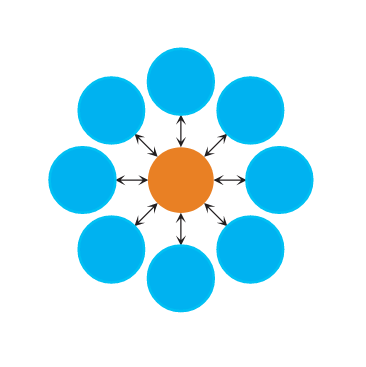
\includegraphics[width=\linewidth]{img/star.png}
        \caption{Star}
    \end{subfigure}
    \begin{subfigure}{.2\textwidth}
        \centering
        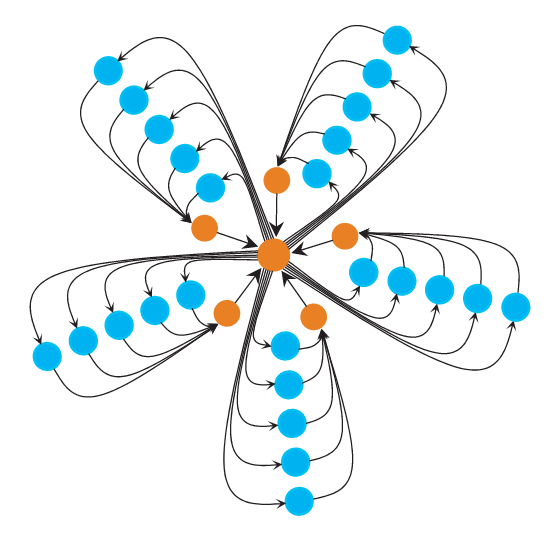
\includegraphics[width=\linewidth]{img/super-star.png}
        \caption{Super-star}
    \end{subfigure}
    \begin{subfigure}{.2\textwidth}
        \centering
        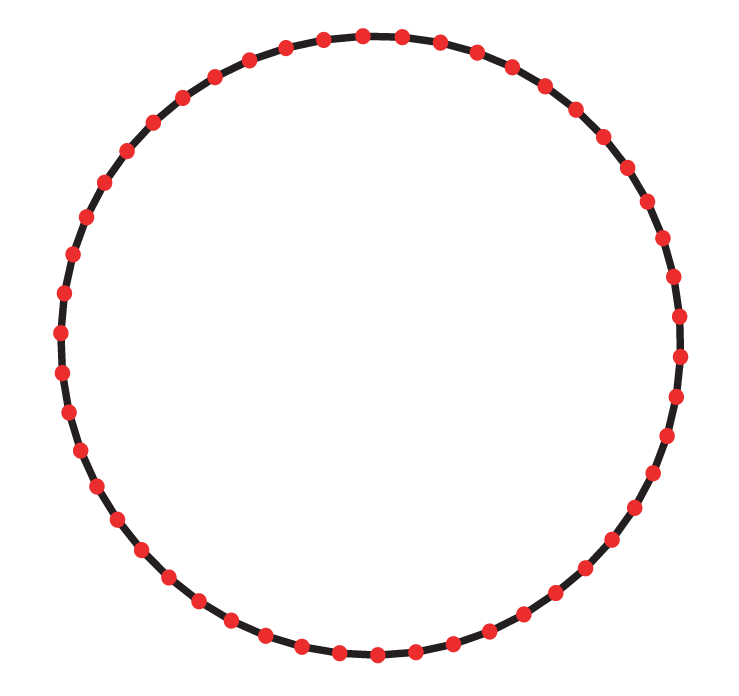
\includegraphics[width=\linewidth]{img/cycle.png}
        \caption{Cycle}
    \end{subfigure}
    \begin{subfigure}{.2\textwidth}
        \centering
        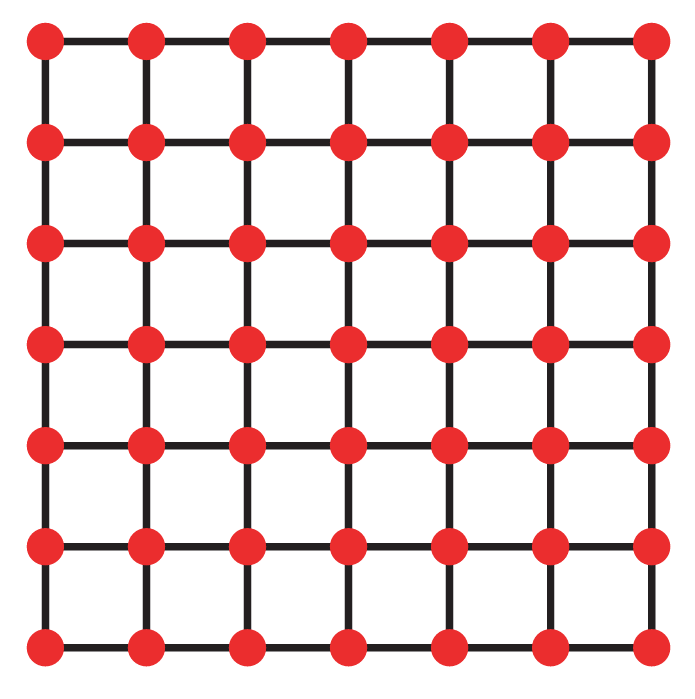
\includegraphics[width=\linewidth]{img/lattice.png}
        \caption{Lattice}
    \end{subfigure}
    \begin{subfigure}{.2\textwidth}
        \centering
        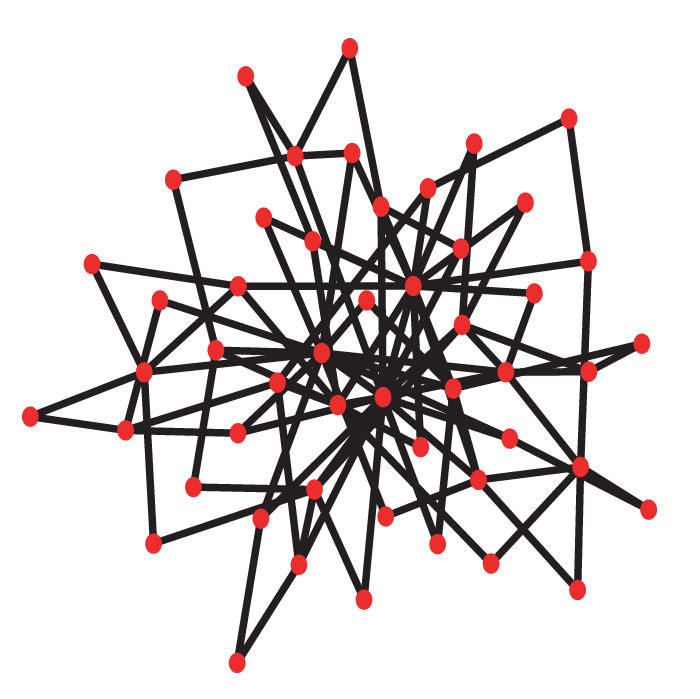
\includegraphics[width=\linewidth]{img/scale-free.png}
        \caption{Scale-free}
    \end{subfigure}
    \caption{\textbf{Different Graph Structures}. Graphs (a) and (b) are reproduced from \cite{liebermanEvolutionaryDynamicsGraphs2005}. Graphs (c)-(e) are reproduced from \cite{ohtsukiSimpleRuleEvolution2006}.}
    \label{diff-graphs}
\end{figure}

In general, calculating the fixation probability of a mutant given its relative fitness is not an easy thing to do. In fact, for most graphs the calculation complexity is NP hard, and so we turn to imposing restrictions on the parameters of the graph.  
\cite{liebermanEvolutionaryDynamicsGraphs2005} found that for a special subset of graphs, named isothermal, the fixation probability relies solely on the relative fitness of the mutant and not the underlying structure of the graph. We say that a graph is isothermal if the sum of the weights of the edges leaving a vertex is equal to the sum of the weights of the edges entering a vertex, hence isothermal. This gives our first theorem. 

\begin{definition}
    An evolutionary graph G is isothermal iff
    \[\sum_j w_{ij} = \sum_j w_{ji} \quad \forall \; v_i\]
\end{definition}

\begin{theorem}
    An EG is isothermal iff the fixation probability of a randomly placed mutant is $\rho_1$.
\end{theorem}

Seeing as this is still a small subset of the total possible graph structures, we turn to alternatives to determing the fixation probability, $\rho$. As mentioned before, we can consider the case when more than one individual mutates and so a subset of the population has fitness not equal to one. 
\begin{definition}
    Let $C\subseteq V$ and $r>0$. Then $P_{C}^{(r)}$ is the fixation probability given that all individuals in $C$ have been replaced with mutants with fitness $r$. 
\end{definition}
Using this definition, we can relate the fixation probability of a subset of a graph to the general fixation probability, $\rho$, using the following equation. 
\begin{equation}
    N\cdot \rho = \sum_{i} P_{v_i}
    \label{eq:sum}
\end{equation}
Going futher, it was found that the subset fixation probabilities are additive under neutral drift, when $r=1$. From Equation \ref{eq:sum} and Theorem \ref{thm:additive}, the fixation probability under neutral drift can be shown to always be $\frac{1}{N}$. Additionally, the fixation probability under neutral drift can be used as a lower bound for determining the fixation probability of an advantageous mutant, $r=1$. Theorem \ref{thm:lowerb} states this formally. 
\begin{theorem}
    Let $r=1$ and $C,D$ be disjoint subsets of $V$. Then $P_C + P_D = P_{C\cup D}$\label{thm:additive}
\end{theorem}
\begin{theorem}
    If $r=1$, then $\rho = \frac{1}{N}$ for all graph structures. 
\end{theorem}
\begin{theorem}
    Let $C \subseteq V$ and $r>1$. Then 
    \[P_{C}^{(1)} \leq P_{C}^{(r)}\] \label{thm:lowerb}
\end{theorem}

While determining the fixation proability of a given mutant has been a central problem in Evolutionary Graph Theory, determining the time to fixation has also been an area of focus. The first main result determined the fixation time for isothermal graphs, the doubly stochastic cases where the sum of the incoming edges is equal to the sum of the outgoing edges at each node. 
\begin{theorem}
    Let $G$ be an isothermal evolutionary graph with large $N$. Then the meant time to fixation for a mutant with fitness $r$ is
    \[t_1 = \sum_{n=1}^{N-1} \frac{(r^N-1)(r^{N-n}-1)(1+r)}{(r^N-1)(r-1)}\]
\end{theorem}
Although it seems to intuitively be true, there still lacks a formal proof for the following conjecture regarding the relationship between the mutant fitness and fixation probability.  
\begin{conjecture}
    The fixation probability, $\rho$, is monotonic with respect to the mutant's fitness, $r$. 
\end{conjecture}





\newpage
\subsection{Games Theoretic Extensions}
Continuing with \cite{shakarianReviewEvolutionaryGraph2012}, we can begin to consider game theoretic extensions of evolutionary graph theory. When considering evolutionary stable strategies in standard evolutionary game theory, the populations are often considered to be well-mixed. We see, however, that considering other population structures leads to different stability results.

Evolutionary stability is a primary focus of evolutionary game theory. A strategy is said to be evolutionary stable if it satisfies two conditions. (1) a population of organisms playing that strategy is resistant to invasion by another strategy and (2) that the strategy is favored by natural selection. (2) is equivalent to saying that the fixation probability, $\rho$, is greater than that of neutral drift, i.e. $\rho > \frac{1}{N}$.

When beginning to examing games on graphs, we first must make a relation between the payoff of the game (P) and the resulting fitness of the organism ($f_i$). This is done with the following equation with parameter $\alpha$. This parameter determines how much influence the payoff of the game has on the fitness of the individual. 
\[f_i = 1 - \alpha+\alpha\cdot P\]

If $\alpha=1$ then the fitness of the organism is equal to the payoff recieved from playing the game. If, however, $\alpha=0$, then the payoff has no effect on fitness. Most applications consider cases of \emph{weak selection}, i.e. where $\alpha <<1$, so that the game has a minimal, but still apparent, impact on the fitness of the individuals.

We begin like all treaties of game theory, with a discussion on the prisoner's dilemma, shown in its normal form below. Two players are offered the choice, simultaneously and independently, to either defect or cooperate. If they both cooperate, they each earn payoffs of 2. If they both defect, they earn a lesser payoff of 1 each. If player 1 chooses to cooperate and player 2 chooses to defect, then player 2 walks away with 3 and player 1 walks away with nothing. Similarly if player 1 chooses to defect and player 2 chooses to cooperate then the first player will walk away with 3 and the second with none.  
\begin{center}
    \begin{tabular}{c | c c }
     & cooperate & defect \\
     \hline
     cooperate & 2,2 & 0,3 \\
     defect & 3,0 & 1,1 \\
\end{tabular}
\end{center}
This game has been studied extensively because of its far-reaching implications in many different fields, especially evolutionary biology. Many species exhibit, and often rely upon, cooperation in their social interactions, but how could this have arisen within Darwin's natural selection framework? Why would an indiviudal choose to cooperate and potentially walk away with nothing? It seems that defectors have the stronger strategy as they can always ensure they walk away with a positive payoff.

In fact, in standard game theory this is the conclusion we reach. Both players are playing their best strategy when they are defecting, corresponding with the formal definition of (defect, defect) being a Nash equilibrium. There is no incentive for either individual to cooperate, so how could that strategy have been favored by natural selection? 

Current evolutionary thoery relies upon Hamilton's rule and the ideas of inclusive fitness. This rule is $rb - c>0$, where $r$ is the relation of an organism to another, $b$ is the benefit, and $c$ is the cost. Thus we have that animals will be expected to cooperate when the benefit outweighs the cost, after accounting for the relationship. 

We can use evolutionary graph theory to divise another rule where organisms are expected to cooperate. We can generalize the Prisoner's dilemma interaction to analzye the influence of the exact benefit and cost relationship. The following table shows the payoffs for the row player in a general cooperative interaction. 
\begin{center}
    \begin{tabular}{c | c c }
     & cooperate & defect \\
     \hline
     cooperate & b-c & -c \\
     defect & b & 0 \\
\end{tabular}
\end{center}
Where $c$ is the cost of cooperating and $b$ is the benefit. \cite{ohtsukiSimpleRuleEvolution2006} found that the condition $b/c > k$ is necessary for the fixation of cooperation, where $k$ is the average number of neighbors. 

 


% Considering a generic two-player two strategy game, this equates to $b < d$. 

% \begin{center}
%     \begin{tabular}{c | c c }
%      & mutant & resident \\
%      \hline
%      mutant & a & b \\
%      resident & c & d \\
% \end{tabular}
% \end{center}

% \cite{tarnitaStrategySelectionStructured2009} found that a mutant strategy is favored over the resident strategy iff $\sigma a + b > c + \sigma d$, with parameter $\sigma$. 

\newpage
\subsection{Numerical Simulations}
Numerical simulations were done in a similar manner to \cite{ohtsukiSimpleRuleEvolution2006}. Graph structures were generated using the $\emph{networkx}$ python package in an Erdős-Rényi manner, but with the added stipulation that the resulting graph be connected \cite{erddsRandomGraphs1959}. The graphs were populated entirely with defectors, then a node was chosen at random to be a cooperator. A Death-birth with death bias update rule was used at each time step. First, nodes played strategic interactions with all of their neighbors, payoffs were calculated, and fitness values updated accordingly with $w=0.01$. Then, the node to die was chosen uniformly from the set of all nodes, and it's strategy was replaced by the strategy of one of its neighbors with probability proportional to its fitness. The graph continued to update in this way until cooperators reached fixation or went extinct. Fixation probabilities were calculated by dividing the number of runs that reached fixation by the total number of runs, $10^5$. Trials were run with a variety of average connectivity and benefit-to-cost ratios. The average connectivity, $k$, was tested with values $3,4,6,8,10$. Nine benefit-to-cost ratios were centered around each value of $k$. For example, for $k=3$, $b/c$ was tested at $1, 1.5, 2, 2.5, 3, 3.5, 4, 4.5, 5$. 

Results are shown in Figure \ref{sim-data} and support the finding the benefit-to-cost ratio rule is necessary but not sufficient for the evolution of cooperation. 

\begin{figure}
    \centering
    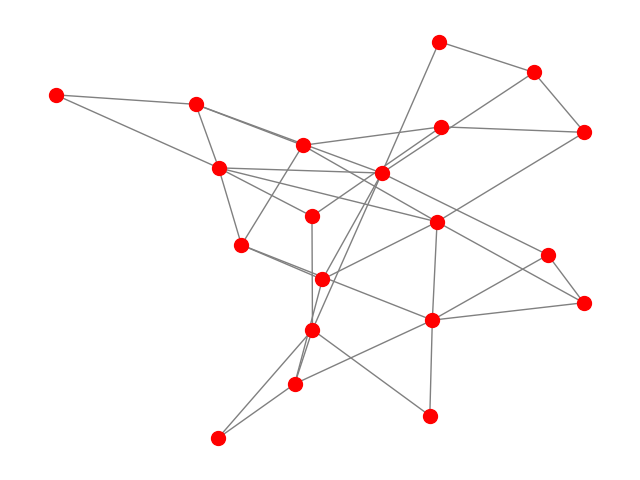
\includegraphics[scale=0.5]{img/random-graph.png}
    \caption{An example of a random connected graph used for simulations.}
    \label{fig:randomg}
\end{figure}
\begin{figure}
    \centering
    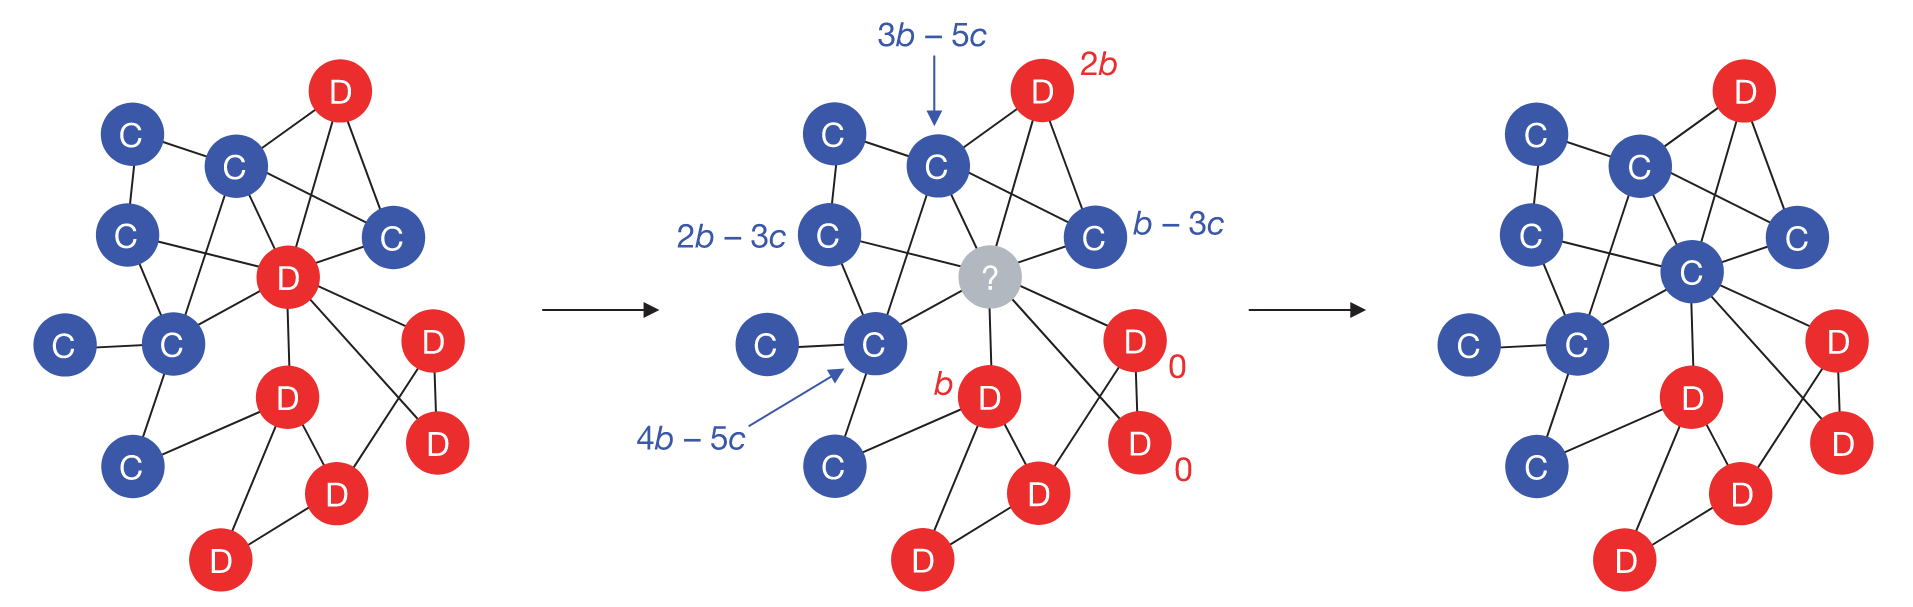
\includegraphics[width=\textwidth]{img/b-c-updating.png}
    \caption{An example of one round of updating. A node is chosen at random to die, payoffs are calculated, and the neighbors are chosen with probability proportional to their fitness to reproduce and replace the node chosed to die. Reproduced from \cite{ohtsukiSimpleRuleEvolution2006}.}
    \label{fig:b-c-updating}
\end{figure}
\begin{figure}
    \centering
    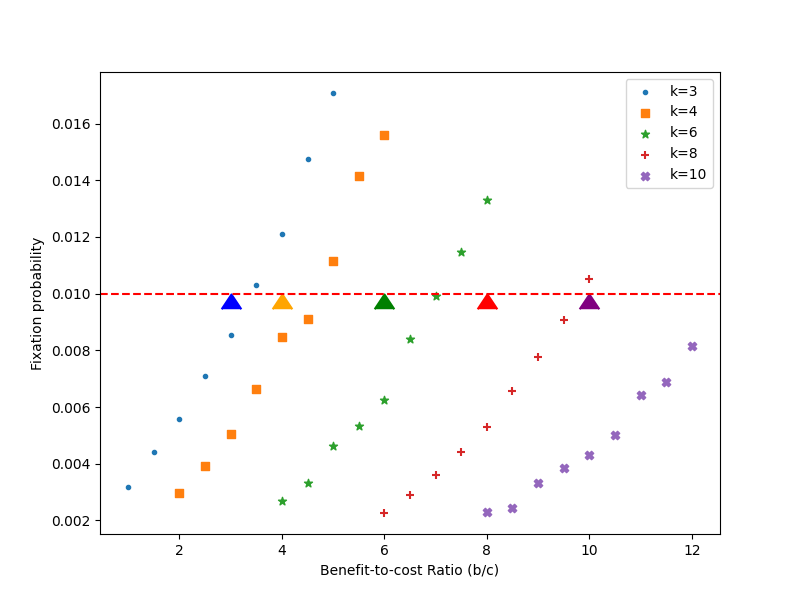
\includegraphics[width=\textwidth]{img/simulation-data.png}
    \caption{\textbf{Simulations support b/c $>$ k rule}: The graph shows the proportion of attempts out of $10^5$ runs that reached fixation, i.e. the number of cooperators reached the total population $N=100$. The average connectivity is represented using $k$ and the benefit-to-cost ratio is given by the x-axis. The dashed line represents the expected number of runs that would reach fixation under neutral drift, $\frac{1}{N} = 0.01$. The triangles mark $b/c = k$. }
    \label{sim-data}
\end{figure}

%    }
\newpage
\bibliographystyle{apalike}
\bibliography{EvolutionaryGraphTheory}


\end{document}
